\chapter{The Java Language Itself}
\pagenumbering{arabic}

\section{JVM内存管理及垃圾回收}
\subsection{运行时数据区组成}
\begin{enumerate}
    \item 程序计数器(Program Counter Register):如果线程执行的是非native方法,则程序计数器中保存的是当前需要执行的指令的地址;如果线程执行的是native方法,则程序计数器中的值是undefined。由于程序计数器中存储的数据所占空间的大小不会随程序的执行而发生改变,因此,对于程序计数器是不会发生内存溢出现象(OutOfMemory)的。
    \item 虚拟机栈(VM Stack):虚拟机栈中存放的是一个个的栈帧,每个栈帧对应一个被调用的方法。当线程执行一个方法时,就会随之创建一个对应的栈帧,并将建立的栈帧压栈。当方法执行完毕之后,便会将栈帧出栈。同理,这也是递归容易导致内存溢出现象的原因。
    \item 本地方法栈(Native Method Stack):Java栈是为执行Java方法服务,而本地方法栈则是为执行本地方法(Native Method)服务。在JVM规范中,并没有对其具体实现方法以及数据结构作强制规定,虚拟机可以自由实现它。在HotSopt虚拟机中直接就把本地方法栈和Java栈合二为一。
    \item 方法区(Method Area):存储每个类的信息(包括类的名称、方法信息、字段信息)、静态变量、常量以及编译器编译后的代码等。
    \item 堆(Heap):用来存储对象本身及数组,堆是被所有线程共享的,在JVM中只有一个堆,因此在堆上分配内存是需要加锁的。
\end{enumerate}

\subsection{判断对象是否存活}
\begin{enumerate}
    \item 引用计数法:给对象头处添加一个引用计数器counter,每当有一个地方引用了对象,计数器加1;引用失效,计数器减1;当计数器为0表示该对象已死、可回收。此方法可能导致循环引用的两个或多个对象都无法进行垃圾回收,例如:
    \begin{minted}{java}
        public class Test {
            public Test ref;

            public static void main(String[] args) {
                Test a = new Test();
                Test b = new Test();
                // a和b交叉引用
                a.ref = b;
                b.ref = a;
                // 将a和b均置为空
                a = null;
                b = null;
                // 手动进行垃圾回收
                // 若采用引用计数法,a, b实则均无法进行垃圾回收
                System.gc();
            }
        }
    \end{minted}
    \item 可达性分析法:首先定义一些对象作为GC Roots,以GC Roots为起点可达对象即为存活对象,不可达对象即为需要回收的垃圾内存。可以作为GC Roots对象的如下:
        \begin{enumerate}
            \item 虚拟机栈中的栈帧的局部变量表所引用的对象。
            \item 本地方法栈中JNI(Java Native Interface)所引用的对象。
            \item 方法区的静态变量和常量所引用的对象。
        \end{enumerate}
        如下图,绿色框起来的部分即为GC Roots,从GC Roots结点出发可以抵达的对象实例有1, 2, 4, 6,对象实例3和5虽然连通,但并没有任何一个GC Roots与之相连,故对象实例3, 5即为需要进行垃圾回收的对象。
        \begin{figure}[h]
            \centering
            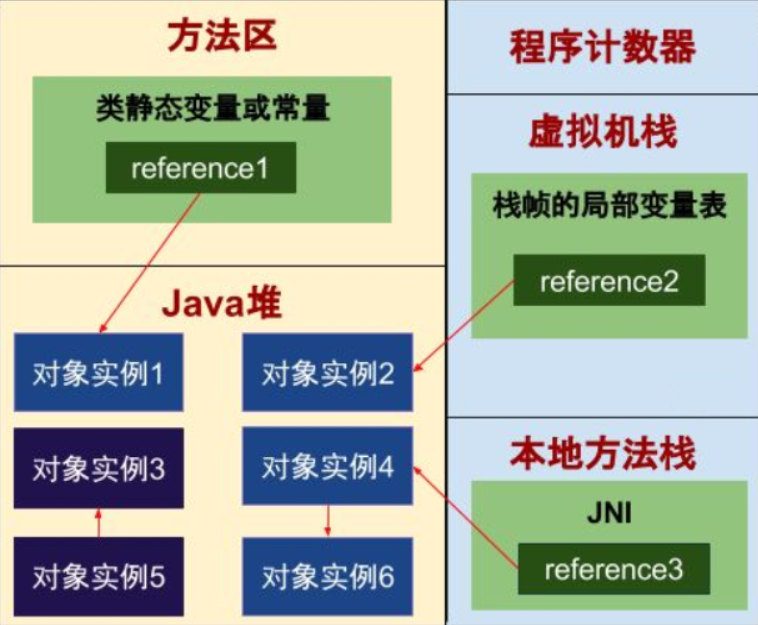
\includegraphics[scale=0.6]{./images/0001.png}
            \caption{Java Memory Model}
        \end{figure}
\end{enumerate}

\subsection{垃圾回收算法}
\subsubsection{标记-清除算法(Mark-Sweep)}
顾名思义,其分为“标记”和“清除”两个阶段:首先标记出所有需要回收的对象,标记完成后统一回收所有被标记的对象。这种算法的不足主要体现在效率和空间,从效率的角度讲,标记和清除两个过程的效率都不高;从空间的角度讲,标记清除后会产生大量不连续的内存碎片,内存碎片太多可能会导致以后程序运行过程中在需要分配较大对象时,无法找到足够的连续内存,而不得不提前触发一次垃圾收集动作,如图:
\begin{figure}[H]
    \centering
    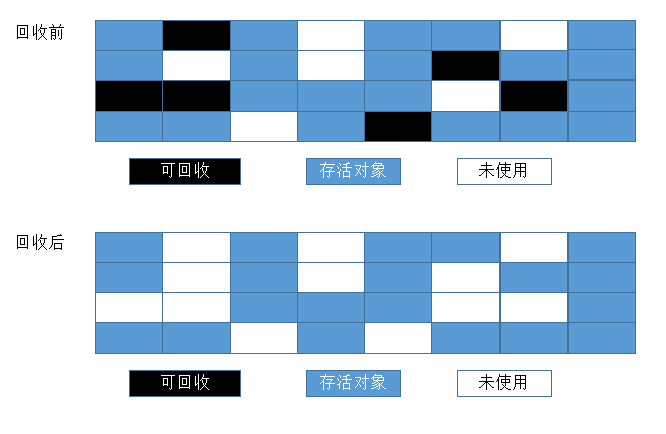
\includegraphics[scale=0.5]{./images/0008.png}
    \caption{Mark-Sweep GC}
\end{figure}
\subsubsection{复制算法(Copying)}
复制算法是为了解决效率问题而出现的,它将可用的内存分为两块,每次只用其中一块,当这一块内存用完了,就将还存活着的对象复制到另外一块上面,然后再把已经使用过的内存空间一次性清理掉。这样每次只需要对整个半区进行内存回收,内存分配时也不需要考虑内存碎片等复杂情况,只需要移动指针,按照顺序分配即可。复制算法的执行过程如图:
\begin{figure}[H]
    \centering
    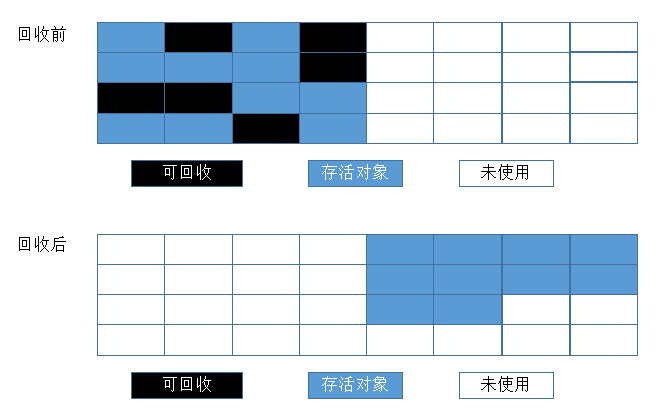
\includegraphics[scale=0.5]{./images/0009.png}
    \caption{Copying GC}
\end{figure}
\subsubsection{标记-整理算法(Mark-Compact)}
让所有存活对象都向一端移动,然后直接清理掉边界以外的内存。如图:
\begin{figure}[H]
    \centering
    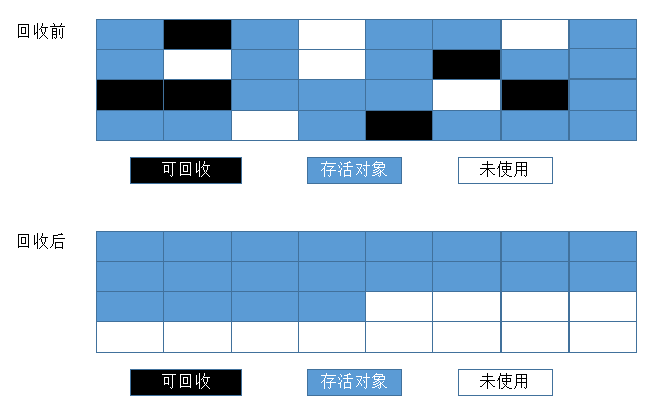
\includegraphics[scale=0.5]{./images/0010.png}
    \caption{Mark-Compact GC}
\end{figure}
\subsubsection{分代收集算法(Generational GC)}
分代收集算法将堆区分为如下几类:
\begin{figure}[H]
    \centering
    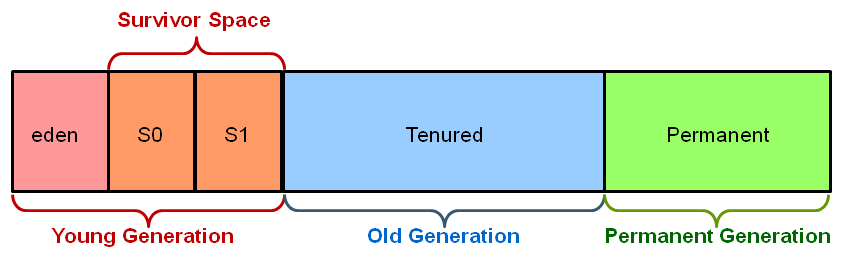
\includegraphics[scale=0.5]{./images/0002.png}
    \caption{Hotspot Heap Structure}
\end{figure}
\begin{enumerate}
    \item 新生代(Young Generation)
        \begin{enumerate}
            \item Eden Space(伊甸园):新对象分配内存的地方。
            \item Survivor Space(幸存者区):Survival区有两块survivor 0和survivor 1。
        \end{enumerate}
    \item 老年代(Tenured Generation):存放存活时间较久的,体积较大的对象。新生代与老年代的比例在1:2左右。
    \item 永久代(Permanent Generation):用于存放一些类的永久数据,JDK8之后不再有永久代。
\end{enumerate}
JVM的内存分配和回收过程如下:
\begin{enumerate}
    \item 所有的新对象都是在eden区进行分配的,两个survivor区在一开始都是空的:
        \begin{figure}[H]
            \centering
            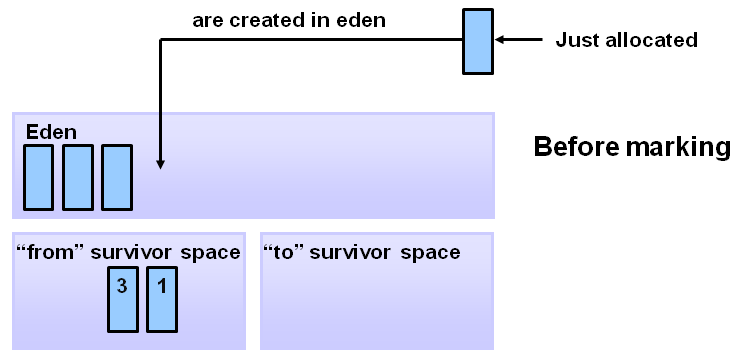
\includegraphics[scale=0.5]{./images/0003.png}
            \caption{Object Allocation}
        \end{figure}
    \item 当eden区满了之后,将会进行一次minor gc。
    \item minor gc时,经引用的对象都会被移动到survivor 0区,未收引用的对象(垃圾清除的目标)将会被直接删除:
        \begin{figure}[H]
            \centering
            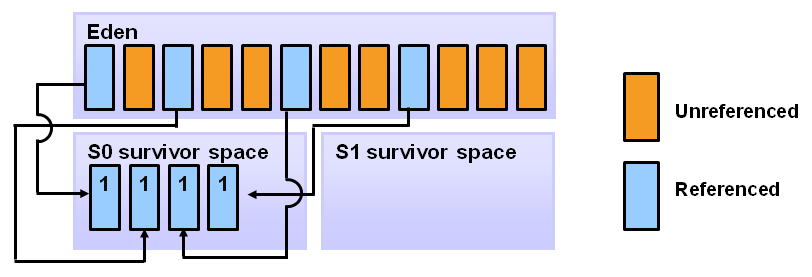
\includegraphics[scale=0.5]{./images/0004.png}
            \caption{Copying Referenced Objects}
        \end{figure}
    \item 再到下一次minor gc时,eden中经引用的对象将会被移动到survivor 1区,目前在survivor 0区的对象,经引用的,将引用计数+1,然后从survivor 0区移动到survivor 1区,未经引用的,将连同eden区一块进行内存释放。经由此过程后,survivor 1区内将会有2中不同年龄(引用计数)的对象:
        \begin{figure}[H]
            \centering
            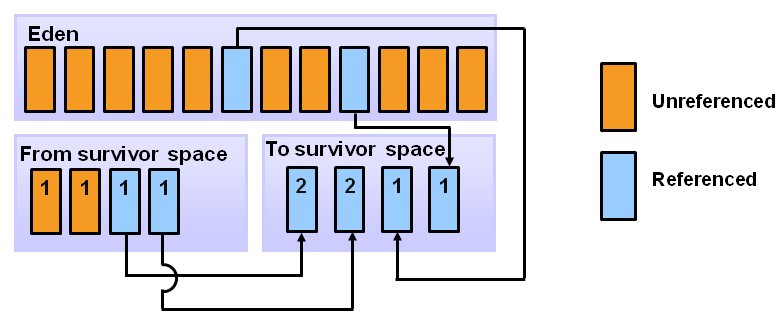
\includegraphics[scale=0.5]{./images/0005.png}
            \caption{Object Aging}
        \end{figure}
    \item 再到下一次minor gc时,eden区和survivor 1区中被引用的对象将会移动到survivor 0区(survivor区互换),然后移动的对象引用计数+1,eden区和survivor1区将会被回收:
        \begin{figure}[H]
            \centering
            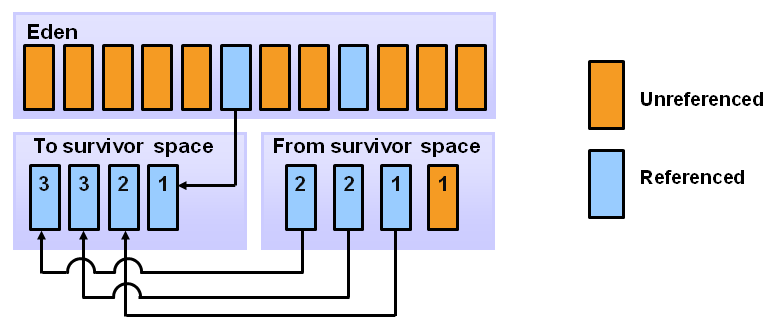
\includegraphics[scale=0.5]{./images/0006.png}
            \caption{Additional Aging}
        \end{figure}
    \item 经过一系列的minor gc之后,一些对象的引用计数将达到设定的阈值(例如8),这些足够老(达到阈值)的将会从新生代移动到老年代:
        \begin{figure}[H]
            \centering
            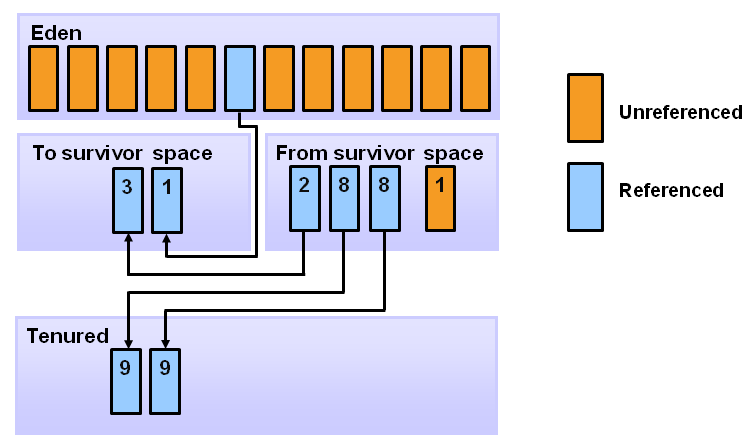
\includegraphics[scale=0.5]{./images/0007.png}
            \caption{Promotion}
        \end{figure}
    \item 当老年代满了之后,会触发major gc(full gc),major gc的发生频率较低,且老年代对象存活时间较长,存活标记率较高。
\end{enumerate}

\section{语言及语法相关}
\subsection{JDK和JRE的区别}
\begin{itemize}
    \item JDK是Java Development Kit,它是功能齐全的Java SDK。它拥有JRE所拥有的一切,还有编译器(javac)和工具(如javadoc和jdb),能够创建和编译程序。
    \item JRE 是Java运行时环境。用于运行已编译的Java程序,包括 Java虚拟机(JVM),Java类库,java命令和其他的一些基础构件,不能用于创建新程序。
\end{itemize}

\subsection{equals、hashCode和==}
==对于基本数据类型比较的是值,对于对象,比较的是对象的堆地址是否相等。Object类中equals()方法底层依赖的是==,默认的Object类中使用equals方法也是对比的对象的堆地址是否相等。hashCode是计算的对象的散列值。三者关系如下:
\begin{enumerate}
    \item 两个对象的hashcode相同,对象不一定是同一个对象。
    \item 两个对象的hashcode不同,那一定不是同一个对象。
    \item 如果两个对象的equals相同,那么hashcode一定相同。
\end{enumerate}
有关String对象的特殊说明,看下面的代码:\\
\begin{minted}{java}
    String a = "ab";
    String b = "ab";
    System.out.println(a == b);
    String c = "a";
    String d = c + "b";
    System.out.println(a == d);
\end{minted}
第一个输出为true,因为"ab"为字符串直接量,同样的字符串直接量将被存储为一个实例,所以a和b都指向一个实例,地址相同,==结果即为true。而a和d的地址不同,所以比较结果为false。而再看这段代码:\\
\begin{minted}{java}
    String a = "ab";
    String b = "ab";
    System.out.println(a.hashCode() == b.hashCode());
    String c = "a";
    String d = c + "b";
    System.out.println(a.hashCode() == d.hashCode());
\end{minted}
首先明确,String类的hashCode值是和其保存的字符串有直接关系的,相同的字符串将会有相同的hashCode值,所以上述代码中,两个地址均输出true。String类型的hashCode计算规则为:\\
\begin{minted}{java}
    s[0]*31^(n-1) + s[1]*31^(n-2) + ... + s[n-1]
\end{minted}

\subsection{泛型中的<? super T>和<? extends T>}
首先,<? super T>表示包括T在内的任何T的父类,<? extends T>表示包括T在内的任何T的子类。你不能往List<? extends T>中插入任何类型的对象,因为你不能保证列表实际指向的类型是什么,你并不能保证列表中实际存储什么类型的对象。唯一可以保证的是,你可以从中读取到T或者T的子类。相反,如果是super就可以写入,因为其基本原则就是,可以将子类的对象赋值给父类,而不可以将父类的对象赋值给子类。同时,List<? super T>往外取时只能放在Object对象里。

\subsection{PECS原则}
PECS即Producer Extends Consumer Super,换句话说,生产者(外界频繁读取数据的)使用<? extends T>,消费者使用<? super T>。简而言之就是:
\begin{enumerate}
    \item 如果你需要从集合中获取类型T,那就使用<? extends T>。
    \item 如果你需要将类型T放入集合中,那就使用<? super T>。
    \item 如果你既要获取又要放置元素,那就不使用任何通配符。
\end{enumerate}
例如在java.util.Collections中的集合复制的方法:
\begin{minted}{java}
    public static <T> void copy(List<? super T> dest, List<? extends T> src) {
        ...
    }
\end{minted}
复制源集合src,主要获得元素,所以用<? extends T>。复制目标集合dest,主要是设置元素,所以用<? super T>。

\subsection{抽象类和接口}
\begin{enumerate}
    \item 接口的方法默认是 public,所有方法在接口中不能有实现(Java 8 开始接口方法可以有默认实现),抽象类可以有非抽象的方法。
    \item 接口中的实例变量默认是 final 类型的,而抽象类中则不一定。
    \item 一个类可以实现多个接口,但最多只能继承一个抽象类。
    \item 一个类实现接口的话要实现接口的所有方法,而抽象类不一定。
    \item 在JDK8中,接口也可以定义静态方法,可以直接用接口名调用。
\end{enumerate}

\section{IO}
\subsection{BIO (同步阻塞IO)}
线程发起IO请求,不管内核是否做好IO准备,从发起请求起,线程一直阻塞,直到操作完成。其根本特性就是做完一件事再去做另一件事,一件事做之前一定要等到前一件事做完。如果线程在执行过程中依赖于需要等待的资源,那么该线程会长期处于阻塞状态,此时处理机就会进行线程的切换,如果在高并发的web或者tcp服务器中系统开辟成千上万的线程,那么处理机的时间就会浪费在线程的切换中,使得线程的执行效率大大降低。

\subsection{NIO (同步非阻塞IO)}
线程发起IO请求,立即返回,内核在做好IO操作准备后,通过调用注册的回调函数通知线程做IO操作,线程开始阻塞,直到操作完成。客户端发送的连接请求都会注册到多路复用器上,多路复用器轮询到连接有IO请求时才启动一个线程进行处理。NIO适用于连接数目较多且连接比较短的架构,比如聊天服务器。\\
NIO的最重要的地方是当一个连接创建后,不需要对应一个线程,这个连接会被注册到多路复用器上面,所以所有的连接只需要一个线程就可以搞定,当这个线程中的多路复用器进行轮询的时候,发现连接上有请求的话,才开启一个线程进行处理,也就是一个请求一个线程模式。

\subsection{AIO (异步非阻塞IO)}
异步非阻塞I/O,服务器实现模式为一个有效请求一个线程,客户端的IO请求都是由操作系统先完成了再通知服务器用其启动线程进行处理。对于读操作而言,当有流可读取时,操作系统会将可读的流传入read方法的缓冲区,并通知应用程序。对于写操作而言,当操作系统将write方法传递的流写入完毕时,操作系统主动通知应用程序。AIO相对于NIO的区别在于,NIO需要使用者线程不停的轮询IO对象,来确定是否有数据准备好可以读了,而AIO则是在数据准备好之后,才会通知数据使用者,这样使用者就不需要不停地轮询了。

\subsection{三者的适用场景}
\begin{enumerate}
    \item BIO:适用于连接数目比较小且固定的架构,对服务器资源要求比较高,并发局限于应用中,JDK1.4以前的唯一选择。
    \item NIO:适用于连接数目多且连接比较短(轻操作)的架构,比如聊天服务器,并发局限于应用中,编程比较复杂,JDK1.4开始支持。
    \item AIO:适用于连接数目多且连接比较长(重操作)的架构,比如相册服务器,充分调用OS参与并发操作,编程比较复杂,JDK7开始支持。
\end{enumerate}

\subsection{同步与异步的区别}
\begin{enumerate}
    \item 同步:发送一个请求,等待返回,再发送下一个请求,同步可以避免出现死锁,脏读的发生。
    \item 异步:发送一个请求,不等待返回,随时可以再发送下一个请求,可以提高效率,保证并发。
\end{enumerate}

\subsection{阻塞与非阻塞的区别}
\begin{enumerate}
    \item 阻塞调用是指调用结果返回之前,当前线程会被挂起,调用线程只有在得到结果之后才会返回。
    \item 非阻塞调用指在不能立刻得到结果之前,该调用不会阻塞当前线程。
\end{enumerate}

\section{Java集合框架}
\subsection{ArrayList和LinkedList的区别}
\begin{enumerate}
    \item 二者都不保证线程安全,但Vector保证线程安全。
    \item ArrayList底层是Object数组,LinkedList底层是双向链表。
    \item ArrayList插入和删除复杂度为O(n),而LinkedList为O(1)。
    \item ArrayList支持快速随机访问,LinkedList不支持。
\end{enumerate}

\subsection{HashMap和HashTable的区别}
\begin{enumerate}
    \item HashMap是非线程安全的,HashTable是线程安全的。也因此HashMap要比 HashTable效率高一点。
    \item HashMap中,null可以作为键,这样的键只有一个。HashTable不支持null作为键,否则抛出NullPointerException。
\end{enumerate}

\subsection{HashMap和HashSet的区别}
\begin{enumerate}
    \item HashSet底层基于HashMap实现。
    \item HashSet实现了Set接口,仅用来存储对象,而不是键值对。
    \item HashSet使用成员对象来计算hashCode值,而HashMap使用key。同步:发送一个请求,等待返回,再发送下一个请求,同步可以避免出现死锁,脏读的发生
    \item HashSet比HashMap慢。
\end{enumerate}

\subsection{HashMap的长度为什么是2的幂次方}
HashMap中的tableSizeFor()方法用来保证HashMap总是使用2的幂作为哈希表的大小。原因是因为经计算出来的hash值需要对数组长度进行取余运算,然后用余数定位其在hash表中的位置,为了优化取余运算的效率,人们发现取余(\%)操作中如果除数是2的幂次则等价于与其除数减一的与(\&)操作,及hash\%length等价于hash\&(length-1),前提是length是2的n次方,采用二进制位操作\&,相对于\%能够提高运算效率。

\subsection{HashMap多线程操作导致死循环问题}
多线程下对HashMap进行put操作会导致死循环问题,原因在于HashMap扩容使用的resize方法,由于扩容是新建一个数组,然后复制原数据到数组,由于数组下标挂有链表,所以需要复制链表,但多线程操作有可能导致环形链表,模拟过程如下:\\
假设当前HashMap的空间为2,hashCode分别为0和1,散列地址为0的地方有元素A和B,这个时候需要添加元素C,经过hash运算,元素C的散列地址为1,这时调用resize方法进行扩容,此时线程1读取到HashMap当前的情况,准备扩容:
\begin{figure}[H]
    \centering
    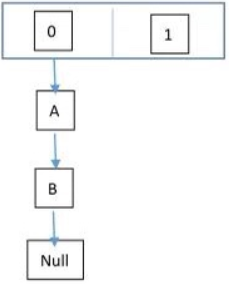
\includegraphics[scale=0.5]{./images/0013.png}
\end{figure}
然后线程2介入,读取HashMap进行扩容:
\begin{figure}[H]
    \centering
    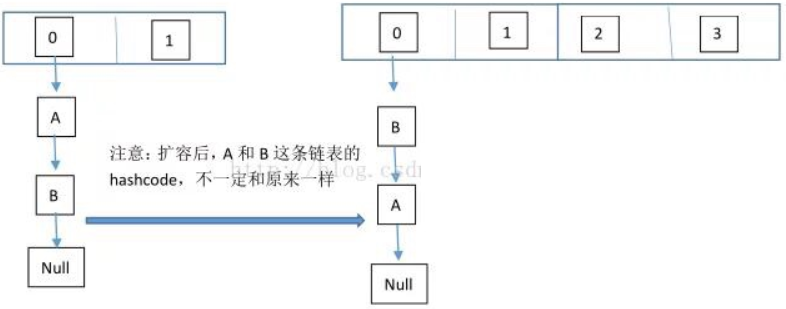
\includegraphics[scale=0.5]{./images/0014.png}
\end{figure}
此后线程1继续执行:
\begin{figure}[H]
    \centering
    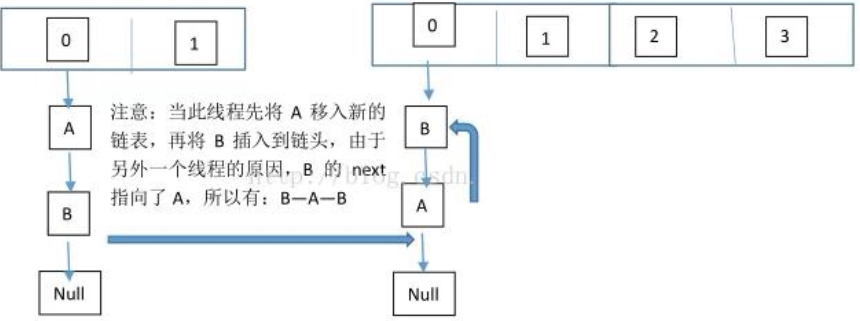
\includegraphics[scale=0.5]{./images/0015.png}
\end{figure}
这个过程为,先将A复制到新的hash表中,然后接着复制B到链表表头(A的前边,即B.next=A),本来 B.next=null,到此也就结束了,但是,由于线程二扩容的原因,将B.next=A,所以,这里继续复制A,让A.next=B,由此,环形链表出现:B.next=A; A.next=B。

\subsection{ConcurrentHashMap线程安全的具体实现方式}
\subsubsection{JDK 1.7}
\begin{figure}[H]
    \centering
    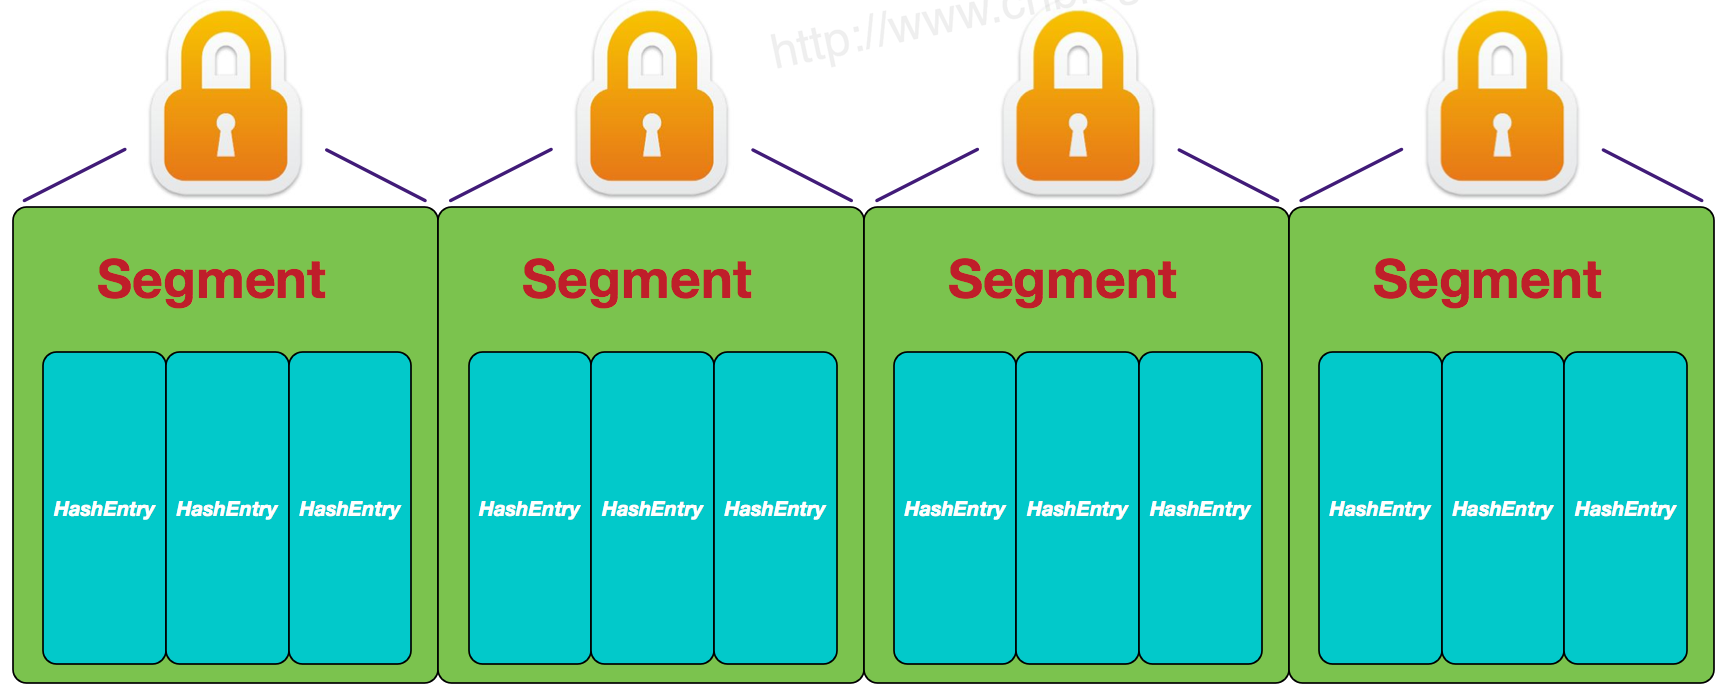
\includegraphics[scale=0.3]{./images/0011.png}
    \caption{ConcurrentHashMap 分段锁}
\end{figure}
使用分段锁来实现线程安全,将数据分为一段一段的存储,然后为每一段数据配一把锁,当一个线程访问占用锁访问一段数据时,其他段的数据也能被其他线程访问。一个ConcurrentHashMap里包含一个Segment数组。Segment的结构和HashMap类似,是一种数组加链表结构,一个Segment包含一个HashEntry数组,HashEntry用于存放键值对数据,每个HashEntry是一个链表结构的元素,每个Segment守护着一个HashEntry数组里的元素,当对HashEntry数组的数据进行修改时,必须首先获得对应的Segment的锁。
\subsubsection{JDK 1.8}
\begin{figure}[H]
    \centering
    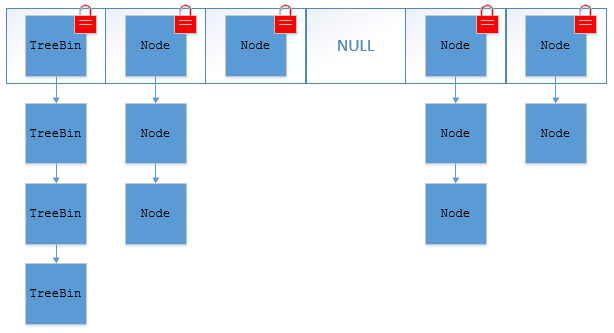
\includegraphics{./images/0012.png}
    \caption{ConcurrentHashMap 分段锁}
\end{figure}
JDK 1.8之后取消了分段锁,采用了synchronized来保证并发安全,synchronized只锁定当前链表或红黑树的首节点,这样只要hash不冲突,就不会产生并发问题。
